% Evaluation plots: pre-rendered PNG (600 DPI), shared grayscale legend.
\begin{figure}[t]
  \centering
  
\includegraphics[width=0.50\linewidth]{Figures/fig2_legend.png}\par\smallskip
  \captionsetup[subfigure]{font=footnotesize,skip=3pt}
  \begin{subfigure}[b]{0.4\linewidth}
    \centering
    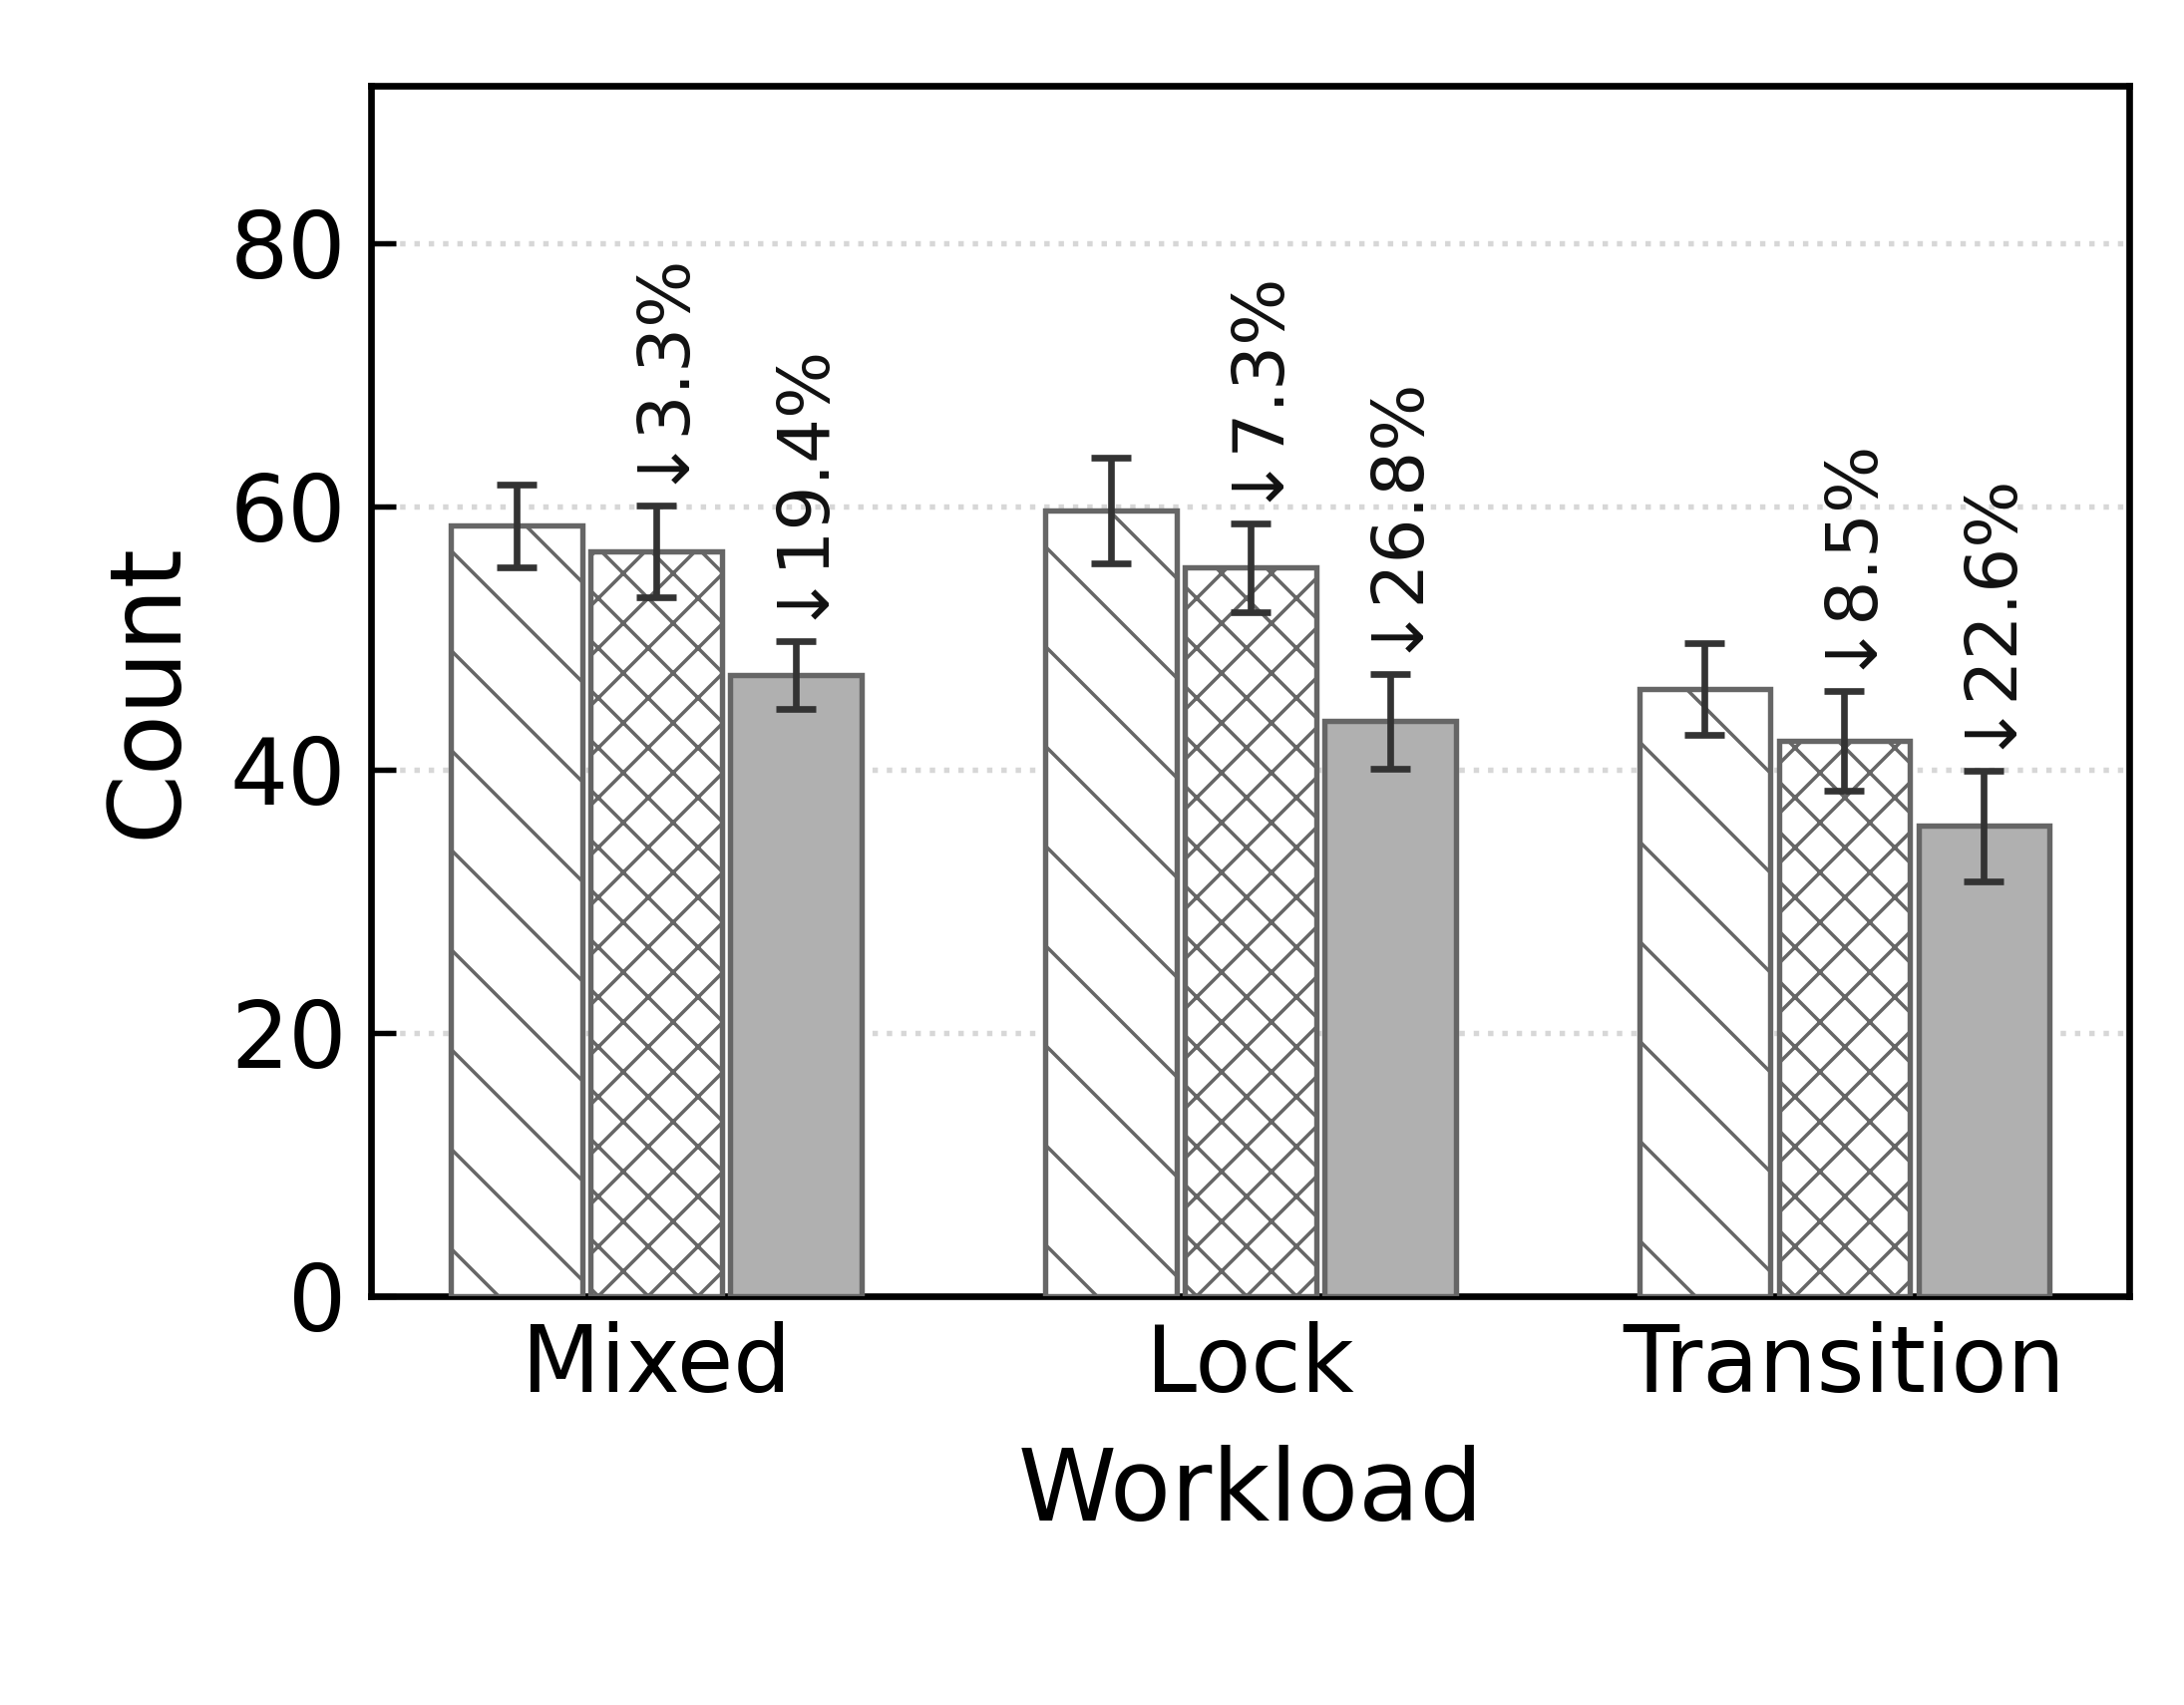
\includegraphics[width=\linewidth]{Figures/fig2_a_deadline_miss.png}
    \caption{Deadline miss}
    \label{fig:sched-deadline}
  \end{subfigure}
  \hspace{2pt}%
  \begin{subfigure}[b]{0.4\linewidth}
    \centering
    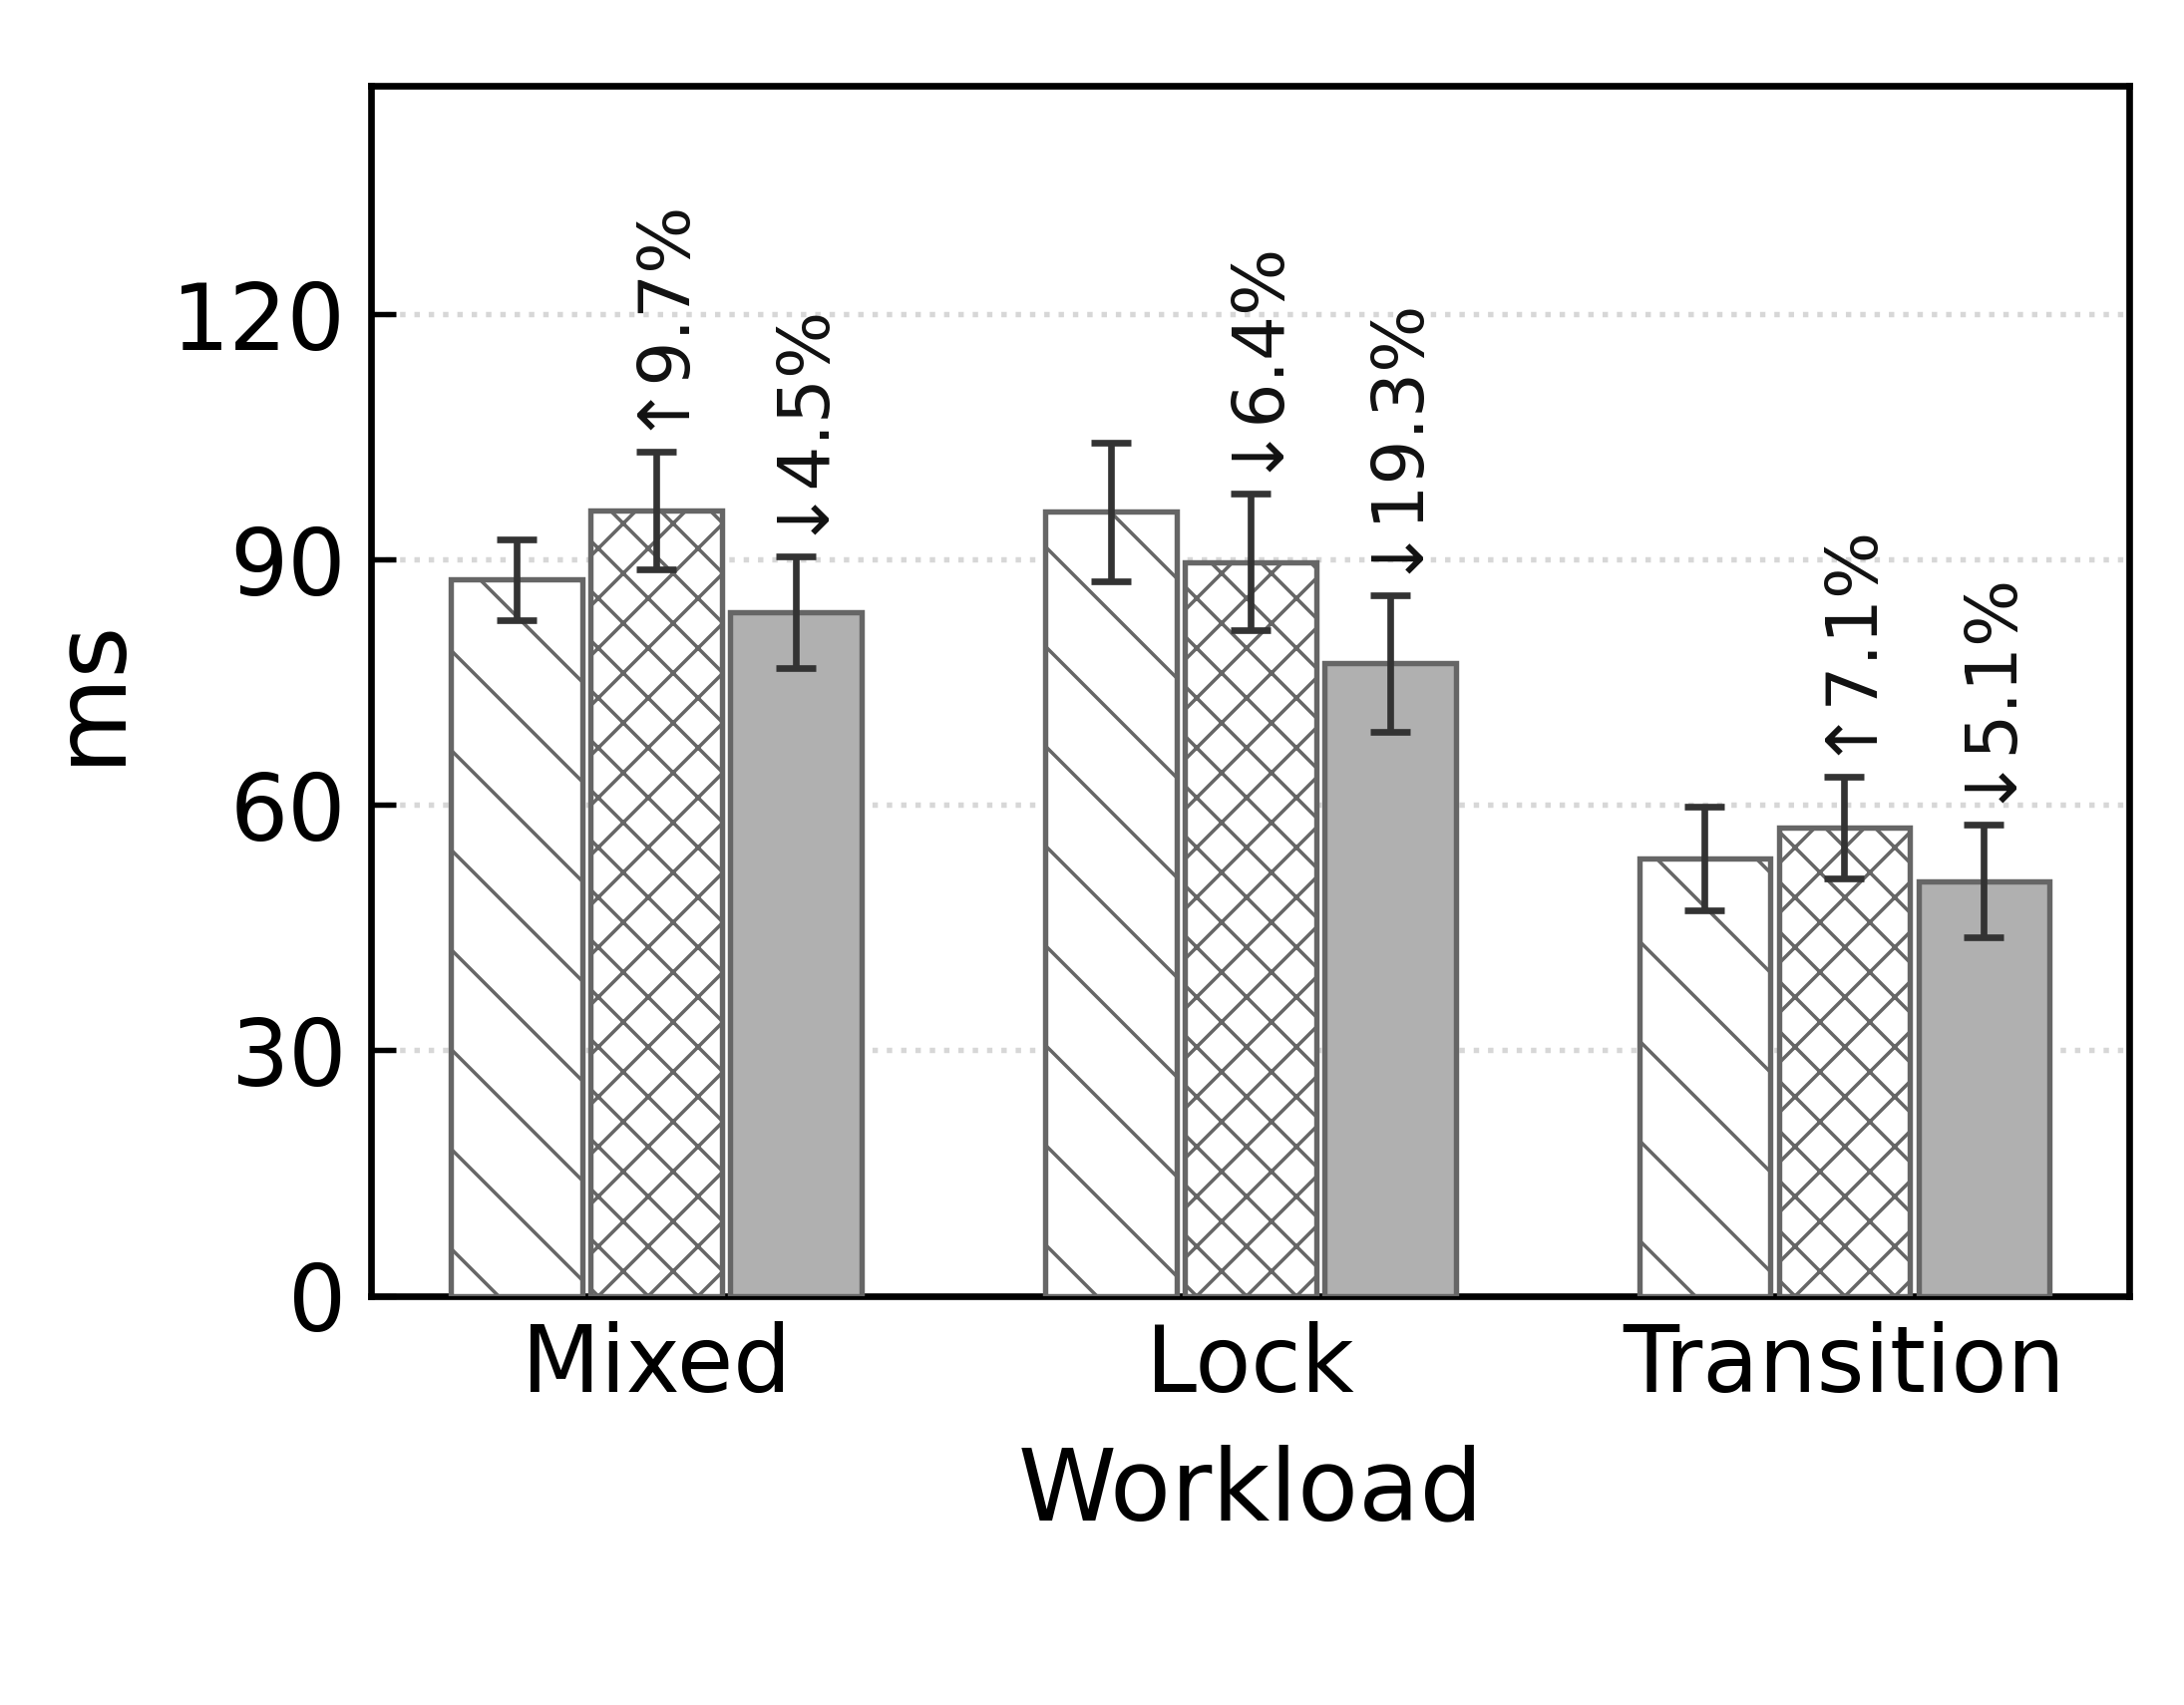
\includegraphics[width=\linewidth]{Figures/fig2_b_deadline_overrun.png}
    \caption{Overrun}
    \label{fig:sched-overrun}
  \end{subfigure}\par\medskip
  \begin{subfigure}[b]{0.4\linewidth}
    \centering
    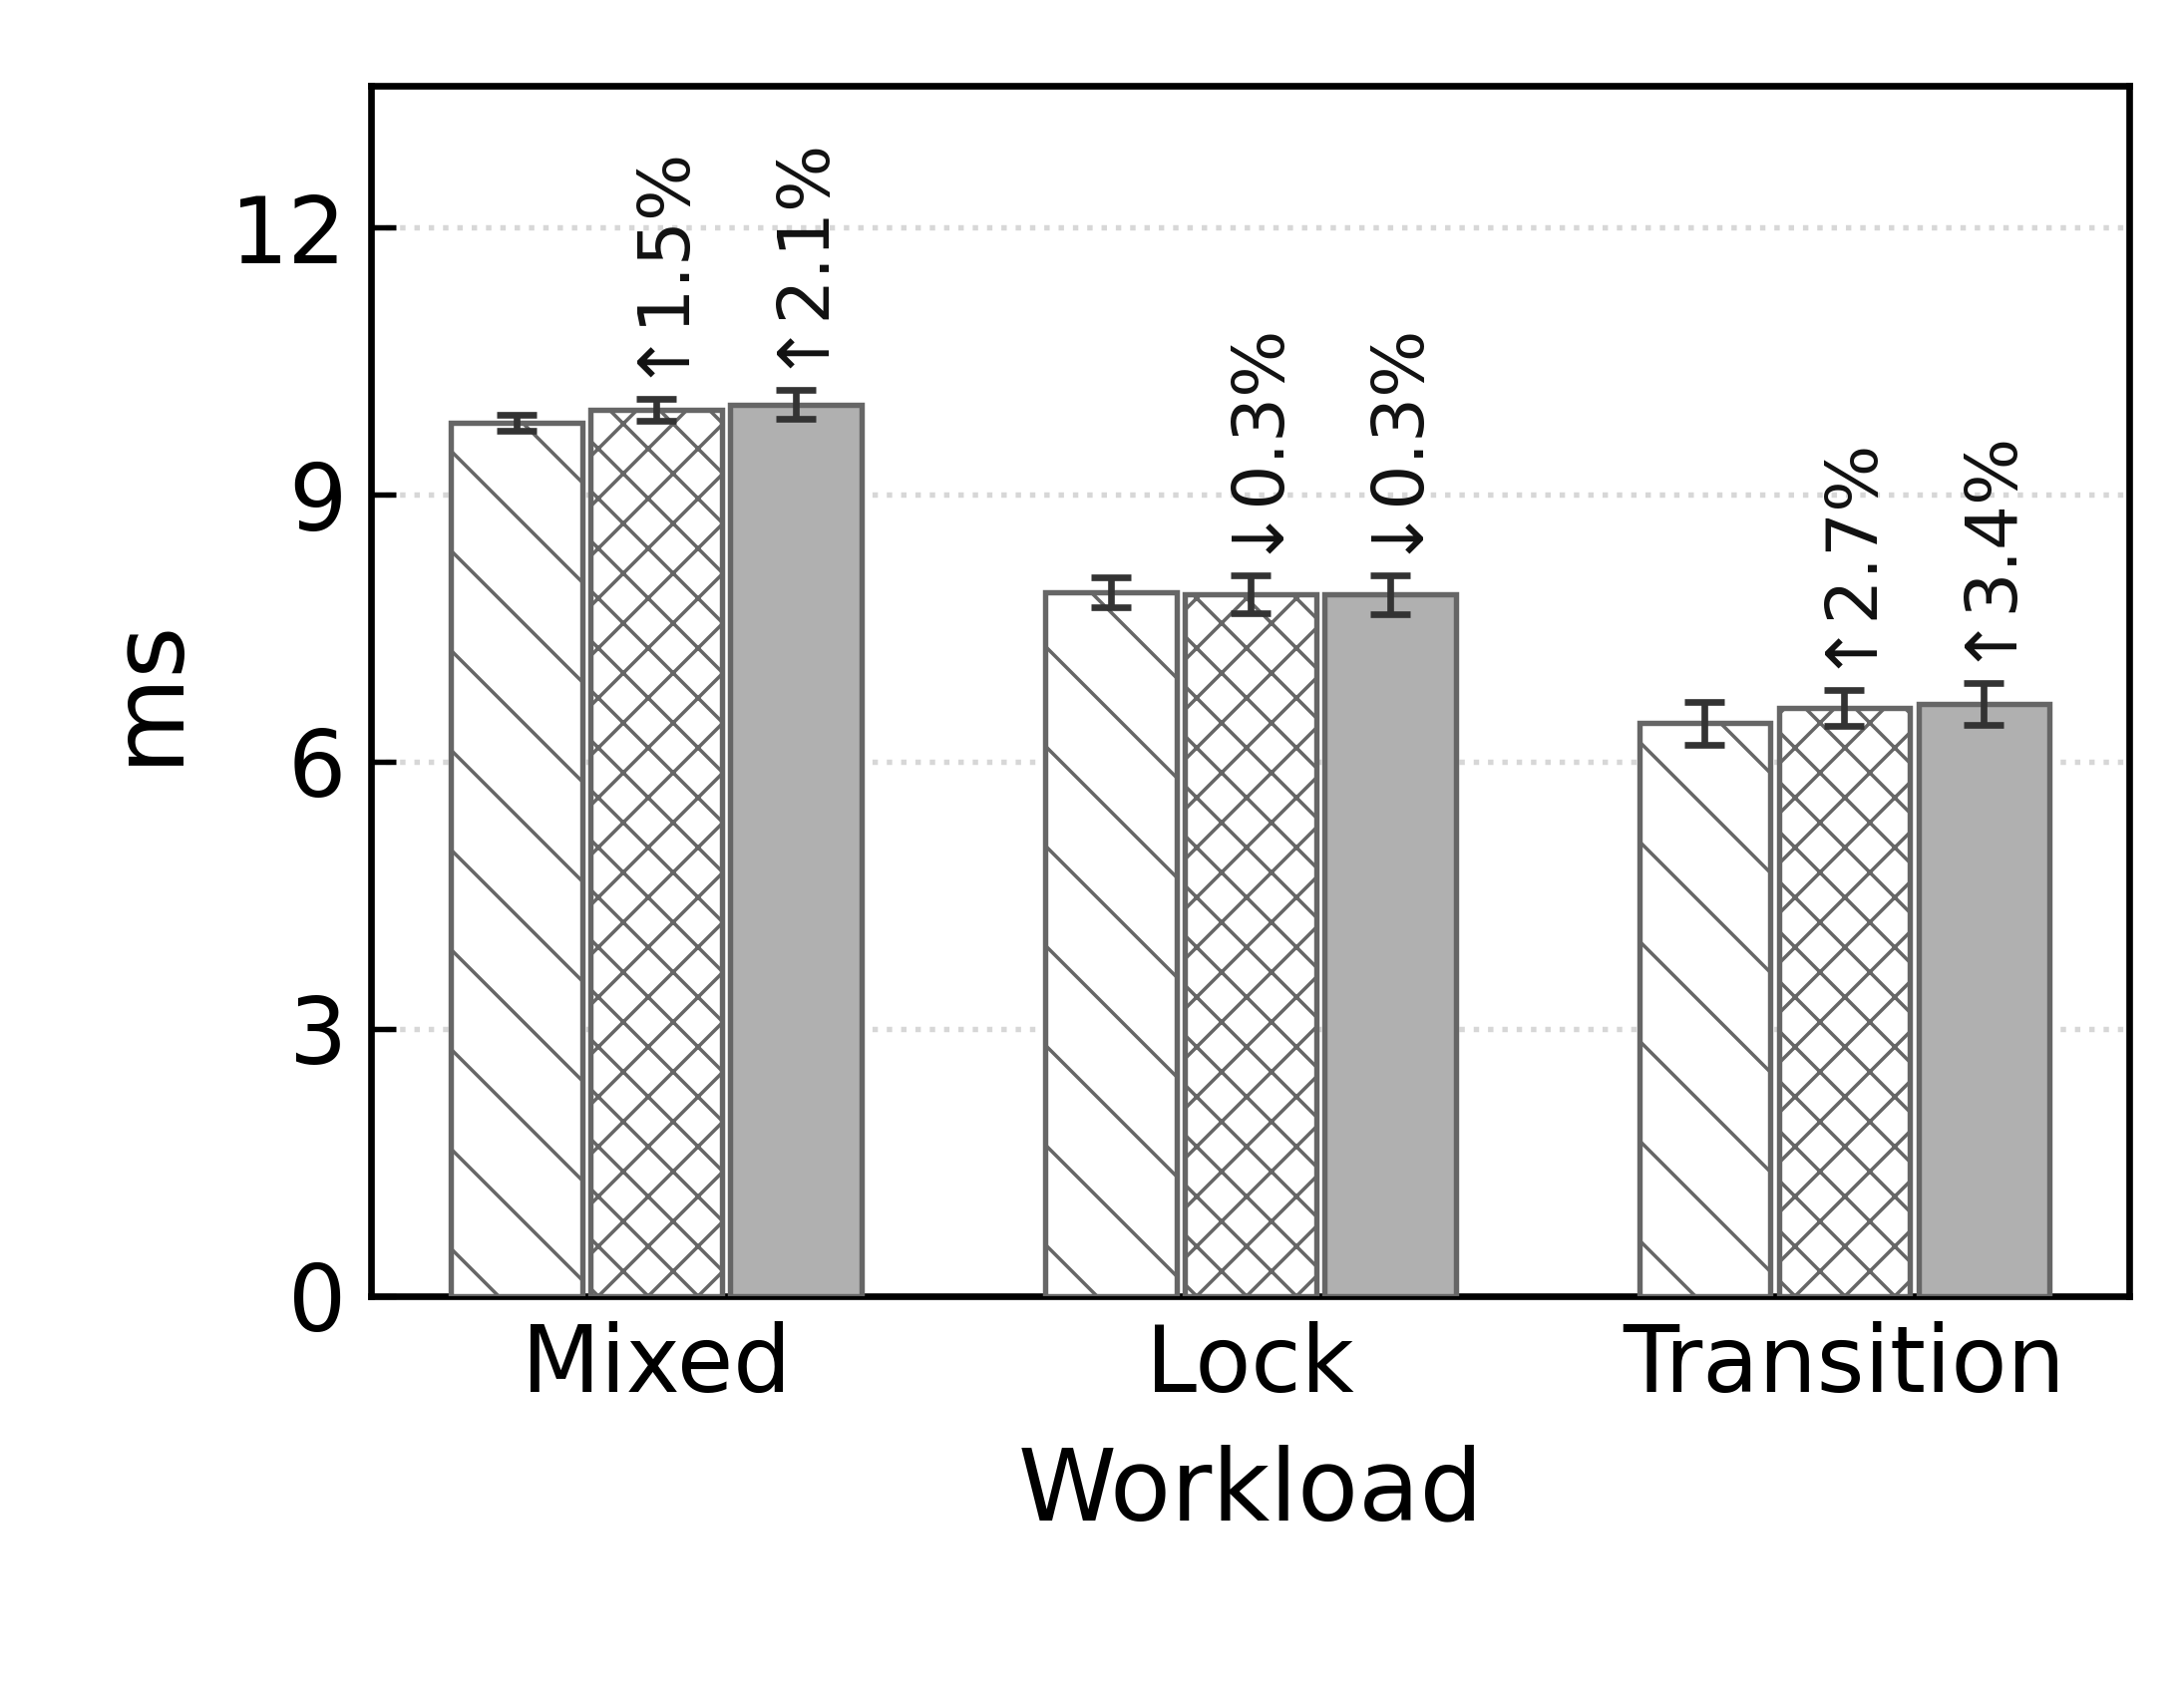
\includegraphics[width=\linewidth]{Figures/fig2_c_request_p99.png}
    \caption{Request p99}
    \label{fig:sched-p99}
  \end{subfigure}
  \hspace{2pt}%
  \begin{subfigure}[b]{0.4\linewidth}
    \centering
    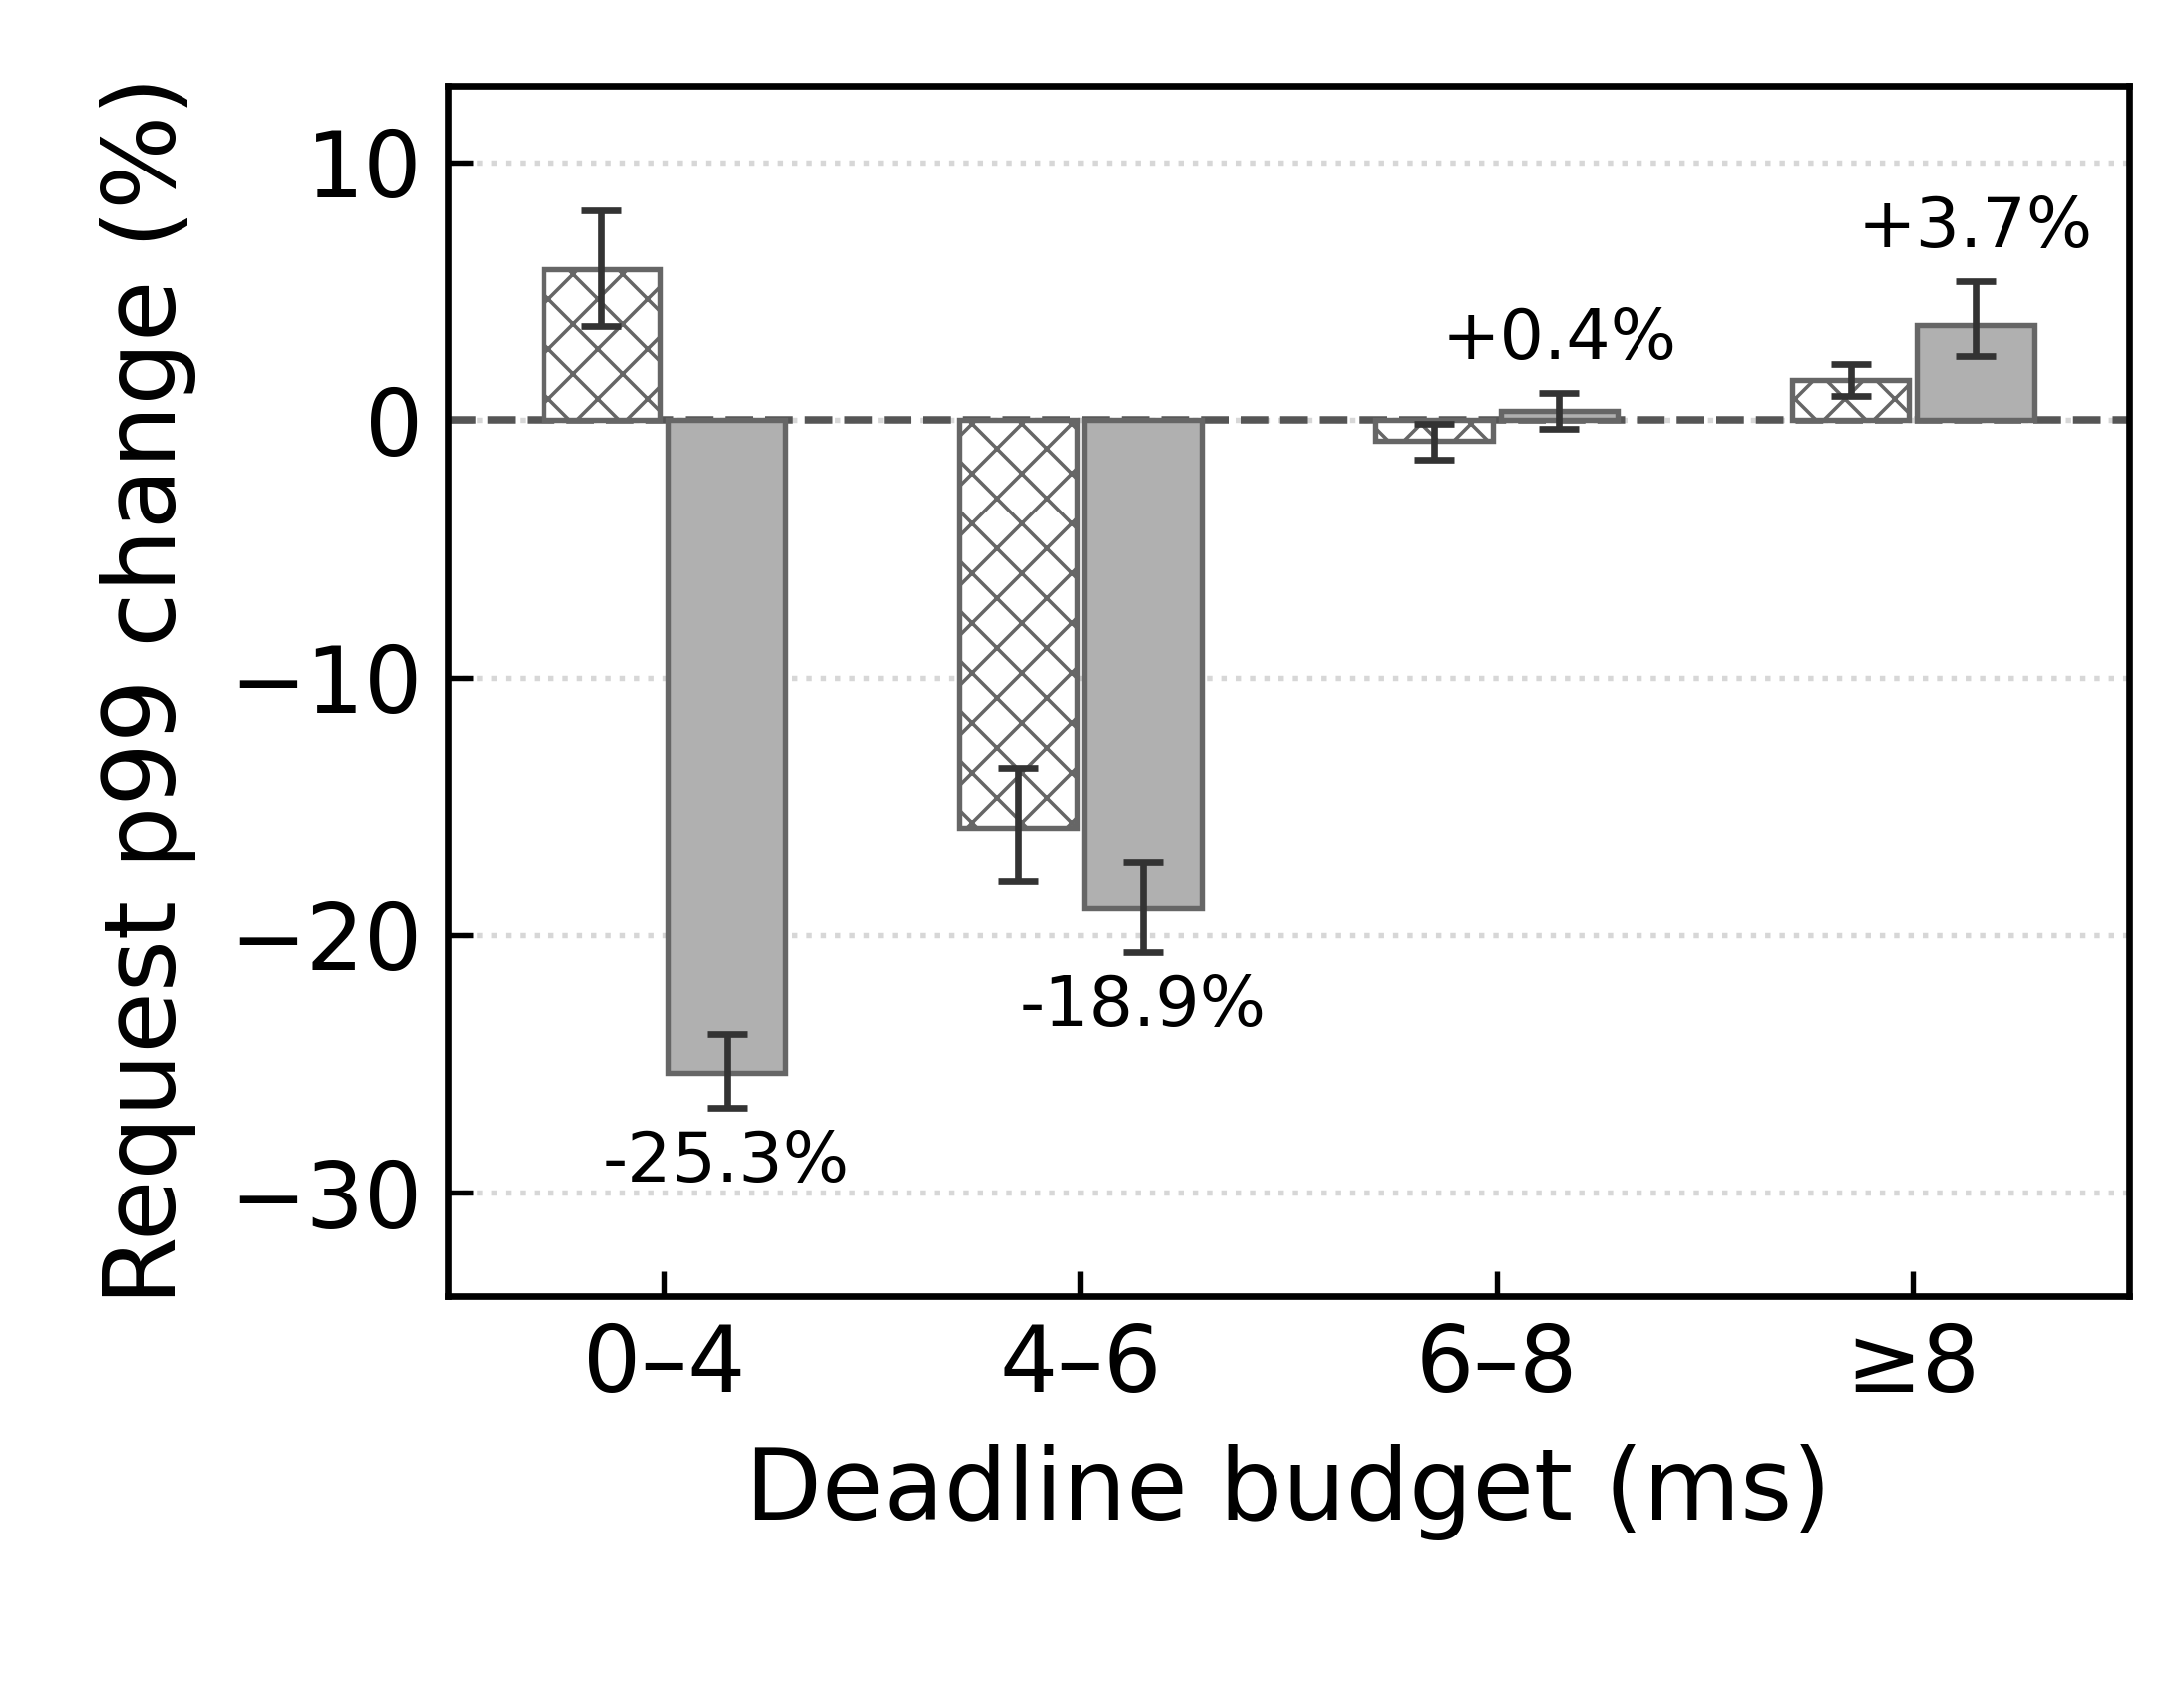
\includegraphics[width=\linewidth]{Figures/fig2_d_mixed_p99_change.png}
    \caption{Mixed p99 change}
    \label{fig:bimodal-p99-budget}
  \end{subfigure}
  \caption{Microbenchmark results on Pixel CPU7. Panels (a)--(c) compare Mixed CPU Bursts (Mixed), Lock Dependency (Lock), and Workload Transition (Transition) using 90 of 100 runs after metric-wise two-sided trimming. Error bars in (a)--(c) denote sample standard deviations. Arrows indicate changes relative to CFS. Panel (d) compares p99 by initial deadline budget in Mixed CPU Bursts using all 100 runs; the dashed line is CFS (0\%), and error bars denote bootstrap 95\% confidence intervals. Negative changes indicate lower latency.}
  \label{fig:sched-microbenchmark}
\end{figure}
